\section{活塞流假设}


\begin{frame}
    \frametitle{流动模型}
    流体在连续反应器中的流动是一种极其复杂的物理现象，而这种现象又直接影响到器内化学反应进行的速率和程度。
    
    流体在管内的径向流速分布是不均匀的，以中心处的流速最大，靠壁处最小。
    \begin{columns}[c]
        \column{5cm}
            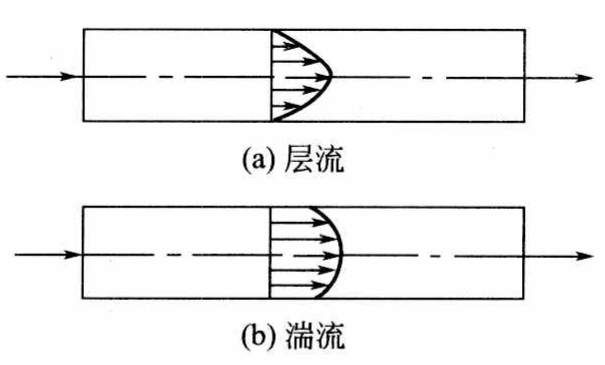
\includegraphics[width=\linewidth]{figs/fig4.1ab.png}
        \column{8.5cm}
            (a) 当流速很小时，流体分层流动，互不混合，称为层流，其径向流速分布为抛物面状；
    
            (b) 当流速增加到很大时，呈湍流，随湍动的程度不同流速分布变得扁平。
    \end{columns}
    显然，中心部分的流体停留时间短，靠近管壁处的流体停留时间则长。停留时间不同，反应程度自然就不一样。

    除了流速分布外，器内的流体混合也是一个极其重要因素。因为流体混合的形式和程度直接影响到器内各处流体的浓度和温度。

\end{frame}


\begin{frame}
    \frametitle{活塞流模型}
    \begin{figure}[h]

        \centering
        
        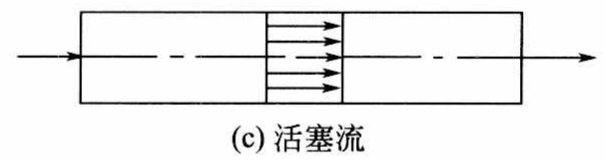
\includegraphics[width=.6\linewidth]{figs/fig4.1c.png}
        
    \end{figure}
    活塞流模型是最基本的一种流动模型。其基本假定如下：    
    \begin{columns}[c]
        \column{0cm}         
        \column{13.5cm}
        \begin{itemize}
            \item[假定1] 径向流速分布均匀；
            \item[假定2] 在垂直于流体流动方向的任何横截面上，浓度均匀，温度均匀，即径向混合均匀；
            \item[假定3] 流体流动方向即轴向上不存在流体的混合，即不存在返混。
            \item[假定4] 由于流体的主体流动和发生化学反应的结果，各个横截面上反应物料的浓度和温度可以是各不相同的。
        \end{itemize}    
    \end{columns}
\end{frame}


\begin{frame}
    \frametitle{全混流模型}

    \large 连续釜式反应器是另一种流动模型，这种流动模型叫做完全混合流模型，简称全混流模型。

    其基本假定是无论径向混合还是轴向混合都达到最大。
    
    最大的径向混合和轴向混合保证了整个反应器内反应物料的浓度均一、温度均一。
    
    活塞流和全混流的根本差别是，前者无返混存在，后者的返混程度则达到最大。

    活塞流和全混流都属于理想化了的流动，所以这两种模型又称为理想流动模型。

\end{frame}